\documentclass[10pt,anonymous,review]{acmart}
\usepackage{wrapfig}

\setlength{\intextsep}{1pt}
\setlength{\abovecaptionskip}{1pt}

\title{Extending Programming with Diagrammatic Programming Languages}
\author{Zac Nowicki}
\affiliation{
  \institution{Kagi Inc.}
  \city{Palo Alto}
  \state{CA}
  \country{USA}
}
\email{znowicki@kagi.com}

\author{Paul Tarvydas}
\affiliation{
  \institution{Retired}
  \city{Toronto}
  \state{Ontario}
  \country{Canada}
}
\email{paultarvydas@gmail.com}

\begin{document}

\begin{abstract}

We assert that DPLs - Diagrammatic Programming Languages - can be used as an adjunct syntax for creating programs.

We give an example of a simple DPL syntax and describe a method for creating executable code using diagrams drawn with off-the-shelf graphic editors.
  
Certain forms of expression are more easily expressed in DPL form rather than TPL - textual programming language - form. TPL-only expression of programs can lead to perceived complexity and other problems. The use of DPLs makes it possible to address these sorts of issues using fresh notations.
\end{abstract}

\maketitle

\section{Introduction - Diagrams as Additional Syntax for Programming Languages}
The goal of programming is to create sequences of instructions -
programs - that cause electronic hardware to perform useful tasks.

To that end, programmers have been employing a single kind of syntax for writing programs -
text.

Use of text for programs was originally based on the early limitations of
electronic hardware and on the convention that the fruits of human thought need to be
expressed as equations written on a two-dimensional medium - paper -
using printing presses.

Early electronic hardware was only capable of supporting grids of
non-overlapping bitmaps called "characters". Today, though, hardware can
support vector graphics and overlapping, resizable windows and widgets of various sizes.

Early electronic hardware strongly encouraged the use of a small number of characters. Programming languages standardized on the use of ASCII, which limited the available number of printable characters to about 96 possibilities.

Early electronic hardware was made to be reprogrammable by the invention of
the Central Processing Unit - CPU. CPUs were originally designed to be
non-reentrant and single threaded. The high cost of early CPU-based
computers prevented use of multiple CPUs in projects, thus, causing the
need for extra software for simulating multiple CPUs on single
hardware devices. Today, though, CPUs - and memory - are inexpensive and
plentiful, a fact which enables the use of alternate forms of
expressing programs. Additionally, the simulation of multiple CPUs via software 
allowed for direct memory sharing between simulated CPUs by default. Physical 
hardware CPUs do not share memory unless such features are specifically 
designed into the hardware. The addition of memory sharing by default in CPU simulations
has been the cause of various kinds of accidental complexity.

The name "CPU" indicates the prevalent notion in early programming, that
hardware designs needed to be controlled by a central authority. This
belief is being strained as hardware becomes more distributed in the
form of internet, robotics, etc. The notion of centrality and
sequentiality was crystallized in early forms of TPL programming,
beginning at least with the FORTRAN\cite{fortran} programming language in 1954.

FORTRAN made the simplifying assumption that CPU subroutines could be
used to express mathematical equations ("formulae"). This assumption was
calcified and led to the invention of the callstack using shared memory.
Preemption was invented when the use of shared memory between
subroutines was found to conflict with the simulation of multiple CPUs.

These early kinds of expression continue to permeate most common
programming languages even today.

This paper shows that these habits of thought can be easily
re-cast using modern hardware and modern software.

This paper describes a technique for extending the syntax of programming
languages.

The new syntax consists of drawings containing simple, closed, graphical
figures and arrows.

We use the the term "DPL" - Diagrammatic Programming Languages - when
referring to this class of new programming syntax.

DPLs might be used \emph{alongside} of existing TPLs (Textual
Programming Languages) and that DPLs are hybrids of diagram and textual
notations. TPLs are useful for expressing a specific kind of program -
computation - whereas other syntaxes make it more fruitful to express
other kinds of programs that don't lend themselves to being expressed in
equation form.

There are multiple possible DPL syntaxes. This paper suggests but a
single DPL syntax. It is assumed that a variety of syntaxes might be
invented, using the techniques described herein.

This paper touches on some of the key aspects of making compilable and
understandable drawings of programs, e.g. 0D, syntactic simplicity, DI
(Design Intent), etc.

We do not discuss fundamental DPL principles in this paper and refer the
reader to other related writings on these subjects.

This paper is laid out in 8 sections.

\begin{enumerate}
\item Introduction - Diagrams as Additional Syntax for Programming
Languages

\item Motivating Example

\item Container and Leaf Components

\item Compilation and Execution

\item Work In Progress

\item Fundamental Principles - describes the basic principles
for convenient development of programs

\item Relevant Principles and Issues - lists various
principles whose discussion is deferred.

\item Future - lists possible avenues for further research.

\end{enumerate}

\section{Example}

  \begin{figure}[h]
    \centering
    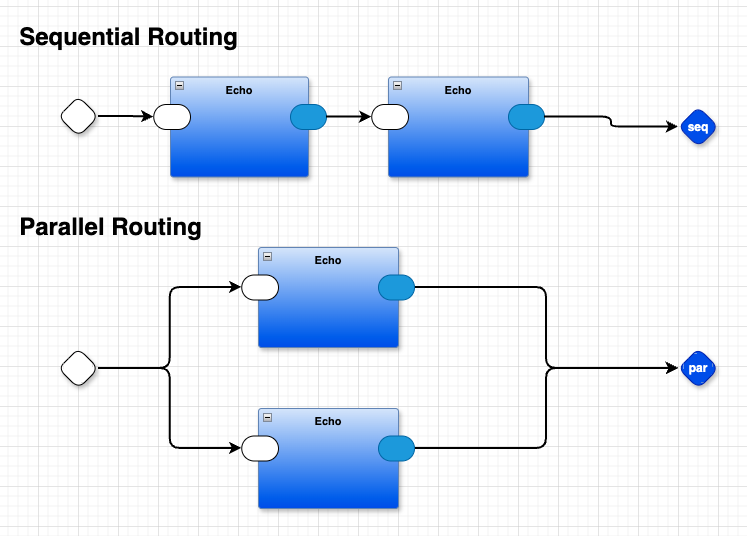
\includegraphics[width=0.8\linewidth]{./media/HelloWorld0D.png}
    \caption{Motivating Example}
    \label{mot}
  \end{figure}

Figure \ref{mot} shows but one sample of a practical DPL syntax. Variations and
improvements on this syntax can be imagined. This syntax is currently being used
to produce actual applications like term-rewriting (\emph{t2t} -
text-to-text - rewriting) compilers, LLMs, DSLs for creating DSLs,
Visual Shell prototypes, games, etc.

This DPL syntax consists of only a few kinds of closed figures plus
arrows plus text associated with the closed figures. Everything else is
considered to be a comment, and, is ignored. For example the bold text
"Sequential Routing" is ignored. Colors are ignored. Line shapes and
line widths are ignored, and so on.

Figure \ref{mot}was drawn using an off-the-shelf diagram editor -
draw.io\cite{diagrams_net}. Draw.io saves the diagram in a modified form of XML, called graphML\cite{graphml}.

The graphML file can be processed using off-the-shelf tools, like an XML parser library or a PEG\cite{peg}-based parser\cite{ohmjs}.

In our case, we used the Odin programming language\cite{odin} and the XML parsing library that is included in the Odin library.

We choose not to reproduce the code for the actual diagram parser here, due to space limitations. The draw.io-specific parser consists of under 250 lines of Odin code (including comments and blank lines). The full source code for the functioning diagram parser is in an open-source repo\cite{d2j}.

\begin{figure}
    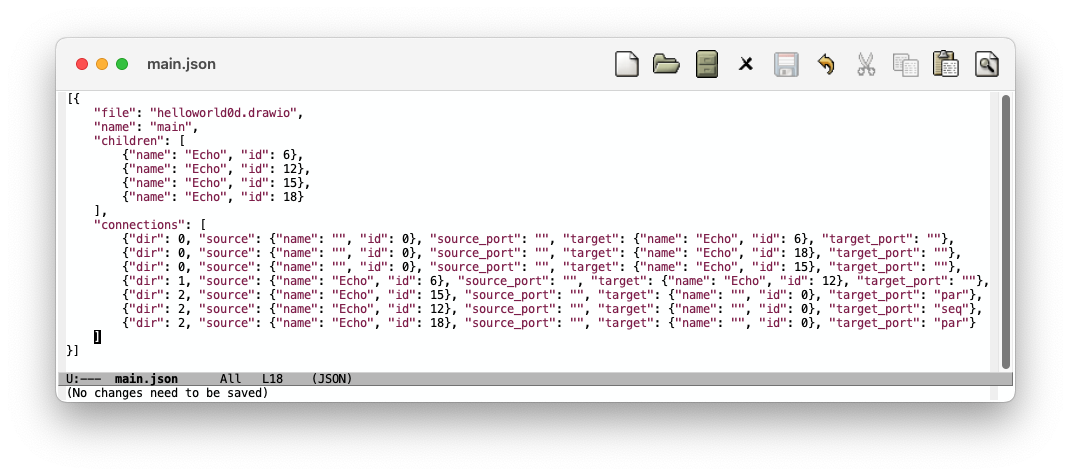
\includegraphics[scale=0.4]{./media/main.png}
    \caption{DPL diagram semantics as JSON}
    \label{main}
\end{figure}
The diagram parser produces internal data structures in the host programming language and/or JSON\cite{json} files.

A \href{http://draw.io}{draw.io} file can contain several diagrams, each on a separate tab (window) in the editor.

The structure of the information needed by the DPL runtime is minimal, consisting of about four (4) fields for each diagram, as seen in Figure \ref{main}:

\begin{enumerate}
\item The filename of the \href{http://draw.io}{draw.io} drawing

\item The tab-name of the top-most diagram.

\item A bag of Children components.

\item A bag of Connections between children (including connections to/from the container itself).

\end{enumerate}

%  \begin{wrapfigure}{l}{0.8\textwidth}
  \begin{figure}
    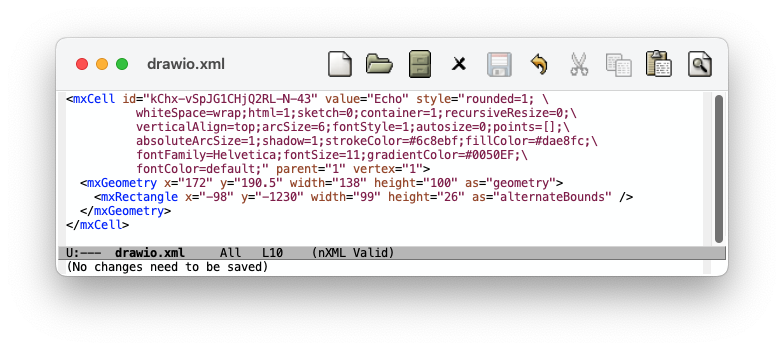
\includegraphics[scale=0.4]{./media/drawio1.png}
    \caption{Raw .drawio}
    \label{drawio1}
%  \end{wrapfigure}
\end{figure}

The .drawio file containing this information is verbose and contains a great deal of graphic layout information that is not relevant at the semantic level.

\emph{The following is simplified for discussion purposes.}

A Child derived from the Echo template is saved in the .drawio file as: (shown with artificial line breaks)

In this DPL, the \emph{style} information is mostly noise from the perspective of semantics. We do need, though, to peer into the style information to determine if the mxCell is a node or a connector (vertex="1" versus edge="1").

%\begin{wrapfigure}{l}{0.7\textwidth}
\begin{figure}
    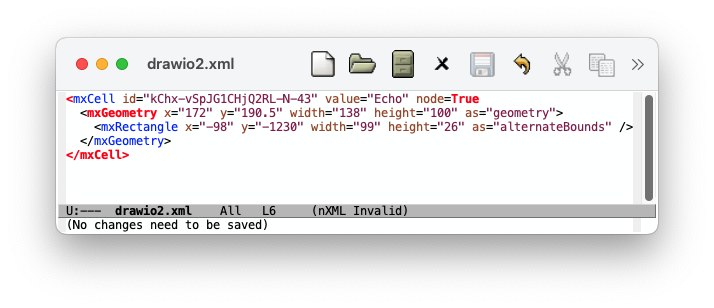
\includegraphics[scale=0.4]{./media/drawio2.png}
    \caption{Cull style noise}
    \label{Darwin}
%\end{wrapfigure}
\end{figure}
When we remove the \emph{style} noise, we get pseudo-XML shown in Figure \ref{drawio2}.

 
\begin{wrapfigure}{l}{0.4\textwidth}
    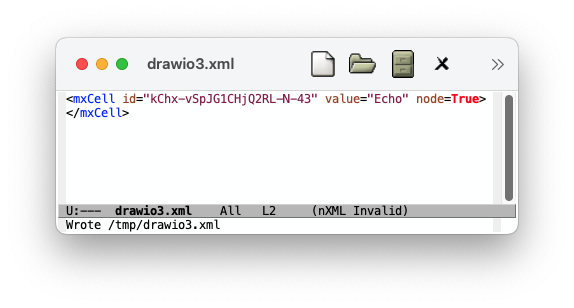
\includegraphics[scale=0.4]{./media/drawio3.png}
    \caption{cull mxGeometry}
    \label{drawio3}
\end{wrapfigure}
Similarly, the \emph{mxGeometry} information affects the visual display of the diagram, but has no semantic value for this DPL.
Figure \ref{drawio3} shows the pseudo-XML after culling the mxGeometry information.
  
\begin{wrapfigure}{l}{0.8\textwidth}
    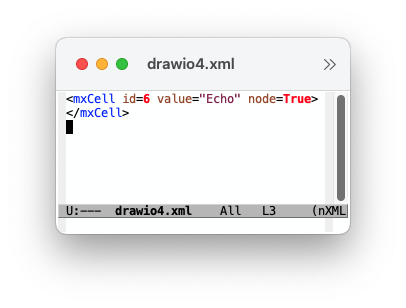
\includegraphics[scale=0.4]{./media/drawio4.png}
    \caption{reduced id}
    \label{drawio4}
\end{wrapfigure}
Furthermore, the id can be internally hashed on a per-file manner, resulting in even less noise:


%%%% JSON snippet
\begin{wrapfigure}{l}{0.3\textwidth}
    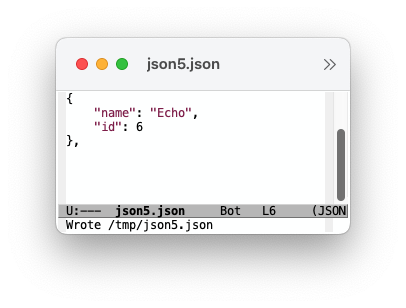
\includegraphics[trim=2cm 2cm 2cm 1.7cm, clip, scale=0.4]{./media/json5.png}
    \caption{Resulting JSON snippet}
    \label{json5}
\end{wrapfigure}
And, from here we can derive the JSON form for a child component

\vspace{1\baselineskip}
All of the above is currently achieved using an XML parser and by cherry-picking information out of
the seemingly-complicated XML data. We argue, though, that this could, also, be replaced
by a PEG parser which performs \emph{t2t} (text-to-text) transformations.

\vspace{5.3\baselineskip}

%%%% IO Ports of 6 culled
\begin{wrapfigure}{l}{0.6\textwidth}
    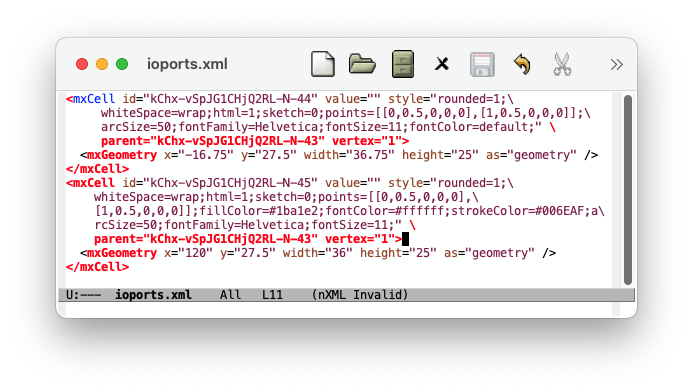
\includegraphics[trim=2cm 2cm 2cm 1.7cm, clip, scale=0.4]{./media/ioports.png}
    \caption{Input and Output Ports of id=6}
    \label{ioports}
\end{wrapfigure}
In this example, the component id=6, derived from the Echo template, has one input port and one output port, seen in Figure \ref{ioports}.

%%%% IO Ports of 6 culled
\begin{wrapfigure}{r}{0.45\textwidth}
    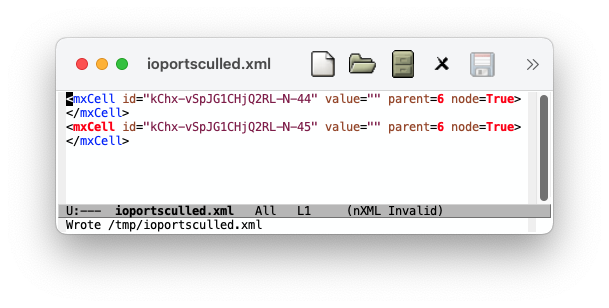
\includegraphics[trim=2cm 2cm 2cm 1.7cm, clip, scale=0.37]{./media/ioportsculled.png}
    \caption{Input and Output Ports of id=6, culled}
    \label{ioportsculled}
\end{wrapfigure}
Here, the ports refer to parent="kChx-vSpJG1CHjQ2RL-N-43" and contain a great deal of graphic information that has no bearing on the semantics.
Culling, we get Figure \ref{ioportsculled}.

Note that "" is a valid port name - the null string. The input port and the output port have the same name (the null string), but, the names do not conflict since they are in different namespaces (input namespace of template "Echo" vs. output namespace of template "Echo").

%%%% Raw Connection
\begin{wrapfigure}{r}{0.45\textwidth}
    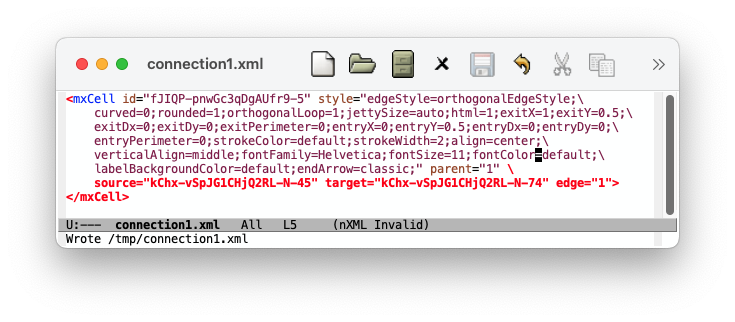
\includegraphics[trim=2cm 2cm 2cm 1.7cm, clip, scale=0.35]{./media/connection1.png}
    \caption{Raw connection}
    \label{connection}
\end{wrapfigure}
Grinding further through the XML, we see several connections, one of which contains a reference to "kChx-vSpJG1CHjQ2RL-N-45". In this case, the reference lists the id as a \emph{source}. This implies that "kChx-vSpJG1CHjQ2RL-N-45" is an output port (there is more nuance to this, but, for simplicity, we'll skip over the nuance for now).


%%%%% Culled connection
\begin{wrapfigure}{r}{0.37\textwidth}
    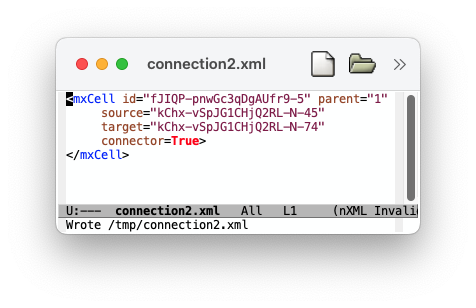
\includegraphics[trim=2cm 2cm 2cm 1.7cm, clip, scale=0.4]{./media/connection2.png}
    \caption{Culled connection}
    \label{connection2}
\end{wrapfigure}
The connection can be culled down to semantically interesting information, as in Figure \ref{connection2}.
Since the source and the targets are children of children of the drawing, the connection is deemed to be of type \emph{across}.
We see these relationships because "...-74" has parent "...-73" which has parent "1" and "...-45" has parent "...-43 which has parent="1". 


\section{Container and Leaf Components} \label{containerleaf}
The diagram in Figure \ref{mot} represents two (2) kinds of components.

The main diagram is, itself, a component. It is a Container which displays its implementation in diagrammatic form as a composition of four other components with connections between them.

Containers can contain other Containers or other Leaf components. In this very simple example, the child components happen to all be Leaf components and, happen to all be derived from the same template - “Echo”. In more practical drawings, this is not usually the case.

Leaf components contain executable code. Leaves do not contain other components.

Children components are drawn as rectangles and contain other, smaller rectangles representing input and output ports for each child component.

Connections are one-way and are drawn as arrows. Line width and style are ignored in this DPL. This allows software architects to choose graphic representations on a per-project basis, emphasizing certain aspects of the design and deemphasizing other aspects. In this example, we use 2pt line thickness to indicate “important” connections. Note that implementing bi-directional connections requires extra software. Bi-directional connections tend to,
also, obfuscate elements of the design.

Input and output ports of the diagram - “gates” - are drawn as rhombuses. 
The kind of each port or gate is determined by how arrows are attached to it. A port that has an arrowhead attached to it is an “input port”, while “output ports” have arrowtails attached to them. Gates, though, are opposite in sense. Gates that have arrowheads attached to them are “output gates” while gates that have arrowtails attached to them are “input gates”.

All rectangles and rhombuses can have one text string associated with them. The text string for components represent template classes. For ports and gates, text strings are tags that are used by components to signify the kind of messages being received and sent. Note that empty strings are legal names and are reserved to mean UNIX®-like standard inputs and standard outputs.

Components in this DPL are completely asynchronous and completely isolated from one another. 

Each component instance - whether Container or Leaf - has exactly one input queue and exactly one output queue.

A key feature of any DPL is that components are truly isolated from one another due to the use of FIFO queues instead of reliance on LIFO callstacks. This conforms with common human understanding of the operation of drawings, objects and actors. Other aspects of DPLs contribute to component isolation, in particular the use of input and output queues and the restrictions on message routing. Components cannot directly send messages to other components. Message routing is handled solely by their parent Containers.

One cannot determine “from the outside” whether a component is a Container or a Leaf, nor know anything about its implementation. One cannot know if a component contains state or is a pure function. In fact, knowledge of these kinds of details is unnecessary. Programmers can dig deeper into the innards of components if they want to know such low-level details.

Components process each incoming message. Processing is based on internal component state and the port tag contained in a message. A message is a 2-tuple \{port, payload\}.

Output message processing consists of placing tagged messages \{tag, payload\} onto the component’s (single) output queue. Output messages are sent in a deferred manner. Output messages sit in a component’s output queue until the component has finished processing one step of its set of potential actions and returns control back to its parent (which is always a Container). The parent container empties a child’s output queue and routes messages in oldest to newest order of output message creation (note that “recursion” works in an opposite manner - most recent first).

Output queues contain messages with port tags that are relative to the \emph{sender}. Input queues contain messages containing port tags that are relative to the \emph{receiver}. Routers, i.e. Containers, must map from output tag of the sender to the appropriate input tags of the receivers.

Component instances need not be explicitly named. Their (x,y) position on a diagram uniquely identifies each instance. Visual placement on the diagram has semantic meaning.


Connections are triples \{direction, sender, receiver\}.


  \begin{wrapfigure}{l}{0.2\textwidth}
    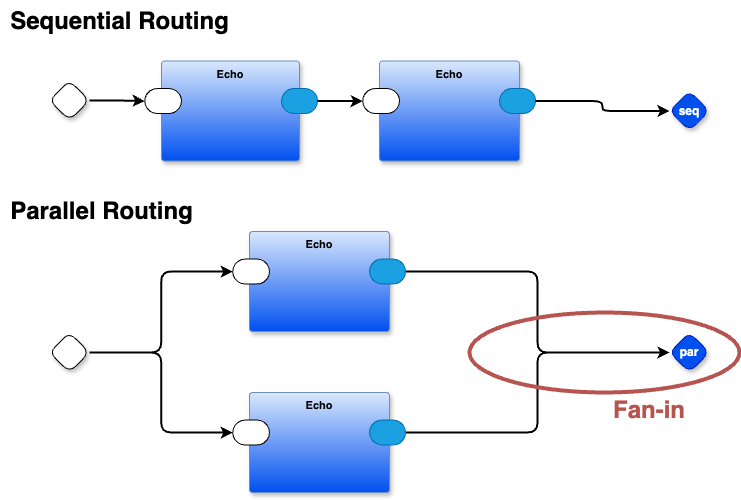
\includegraphics[scale=0.1]{./media/fanin.png}
    \caption{Fan In}
    \label{fanin}
  \end{wrapfigure}

Fan-in and fan-out are supported. Fan-in means that a single input port/gate can receive messages from multiple sources. This is straight-forward to implement using the FIFO queue structure of components. Fan-out, though, means that a single port/gate can send messages to several receivers. This requires copying of message payloads or the application of copy-on-write semantics in the receivers. There is no semantic difference between these two techniques - the choice of implementation (copying vs. copy-on-write) is purely one of optimization and does not matter at the design stages. Efficiency of implementation matters only during Production Engineering stages, i.e. when a design is stable enough to be productized.

In Figure \ref{fanin} the output gate "par" shows fan-in, as it receives inputs from two different component instances. The outputs from the two "Echo" instances do not collide. The outputs are queued up on the diagram's output queue in the order that they were generated.


  \begin{wrapfigure}{r}{0.2\textwidth}
    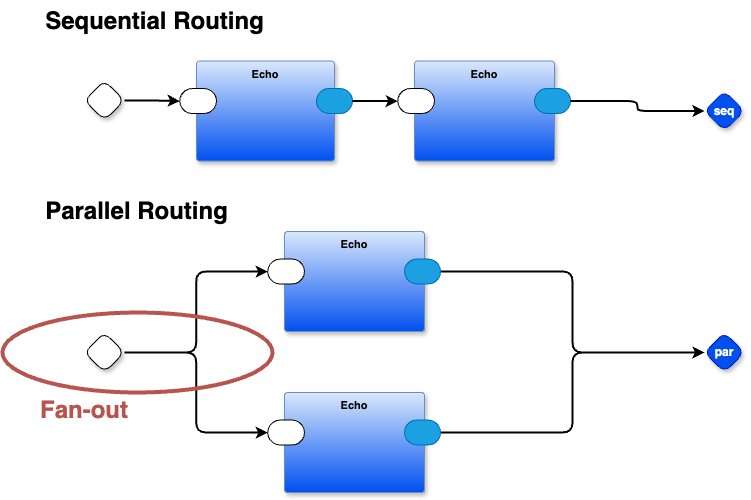
\includegraphics[scale=0.1]{./media/fanout.png}
    \caption{Fan Out}
    \label{fanout}
  \end{wrapfigure}
The corresponding input gate demonstrates fan out in Figure \ref{fanout}. Any message on the input gate is routed to both instances of the "Echo" component on the "Parallel Routing" subnet.


Furthermore, fan-out requires atomic routing. A single output message must be delivered to all receivers in an atomic fashion without allowing interleaving messages to arrive from other sources. This requirement ensures that messages are queued in a consistent manner relative to one another. The actual, absolute timestamp of any message does not matter, and the final order of messages does not matter, but message relative-order does matter. If “A” arrives before “B” at one receiver, then, “A” must arrive before “B” at \emph{all} receivers. Physics informs us that, ultimately, we cannot tell if “A” arrived before “B” or if “B” arrived before “A”, and that this is the only real “race condition”. Programmers can deal with that single kind of “race condition” as long as message-relativity is preserved. In general, though, message relativity cannot be preserved across large distances (“A” might arrive before “B” at one receiver, but, “B” might arrive before “A” at another receiver because “B” has less-far to travel). Preserving message relativity in-the-small, inside a single application, makes it easier to write such application programs. Note that this DPL is “yet another notation”, like function-based programming, which can simplify programming in many cases, but, cannot be used in \emph{all} cases.

Fan-in and fan-out, also, apply to inter-component connections (\emph{across} connections).

Fan-out may be an inconvenience in the theoretical sense, but, is a vital feature for usability of DPLs. For example, fan-out makes it possible to abstract diagrams by grouping components together and pushing them over onto other diagrams, leaving only a single component with fewer ports on the originating diagram. This kind of usage is fundamental to one’s being able to layer a design in meaningful ways. In contrast, function-based programming relies on a single expression for layering - the function (aka “lambda”). The paucity of expression in function-based-only-programming leads to obfuscation of design intent (“DI”) and makes designs appear more complicated than necessary to casual readers. A simple example of fan-out can be seen in Figure \ref{fanout} where only one input gate is needed to feed two separate input ports.




In this DPL, there are four (4) connection directions
\begin{itemize}
\item down
\item across
\item up
\item through.
\end{itemize}
The sender information in connections must include a reference to a component instance and a port.
The receiver information in connections must include a reference to a component instance and a port.
As already mentioned, mapping from sender-ports to receiver-ports must be done by parent containers during the process of message routing.
\subsection{Container Component}
Each diagram is compiled into a container component containing the following information:
\begin{itemize}
\item template name - the name of the diagram
\item bag of children 2-tuples \{template, instance-id\}
\item bag of connection 3-tuples \{direction, \{sender, port\}, \{receiver, port\}\}
\end{itemize}

%%%% Echo
\subsection{Leaf Component "Echo"}
\begin{wrapfigure}{r}{0.5\textwidth}
    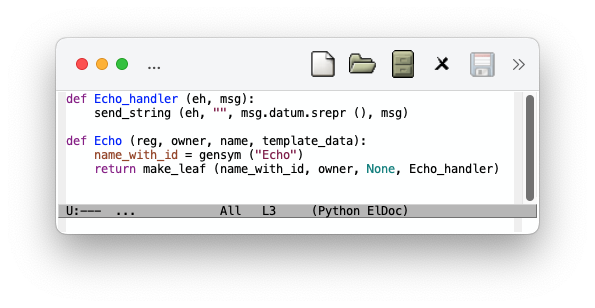
\includegraphics[trim=1.7cm 2cm 1.7cm 1.5cm, clip, scale=0.4]{./media/echo.png}
    \caption{Echo}
    \label{fig:echo}
\end{wrapfigure}
In our implementation, we used the Odin programming language for
creating the diagram parser, but, we use the Python programming
language to load and execute the parsed results.

Figure 1 refers to a Leaf component template called "Echo". The "Echo"
component is instantiated three (3) times. 

Leaf components are
implemented with code in some host language (Python, in our case) as in Figure \ref{fig:echo}. Software components
appear as rectangles on the drawing. The implementation provides two (2)
entry points for each software component:
\begin{itemize}
\item The code to instantiate a component from the "Echo" template. In Figure
1, the "Echo" code creates three (3) instances, each being unique, but,
derived from the same template.

\item The code to handle incoming messages for each instance derived from the
template. In this example, an "Echo" component does nothing more than
forwarding the received message. The \emph{handler} code is activated for
\emph{each} incoming message.
\end{itemize}

\section{Compilation and Execution}
Compilation and execution of this DPL consists of the steps listed below. Note that the diagrams are rough sketches intentionally simplified
for overview purposes only.

\subsection{Convert DPL program diagrams to JSON.}

%  \begin{figure}[h]
%    \centering
%    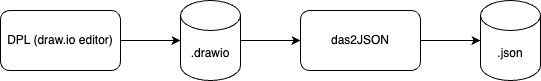
\includegraphics[width=0.6\linewidth]{./media/convert.png}
%    \caption{Convert diagram to JSON}
%    \label{fig:convert_to_json}
%  \end{figure}

  Transpilation of the diagrams (XML) into JSON (or internal data structures, if efficiency is at a premium). The diagrams represent \emph{templates} for components.
  
  In our implementation, \texttt{das2json} is implemented\cite{d2jrepo} in the Odin programming language. The process begins with a straightforward call to the XML parsing library. The XML data is then deconstructed into a convenient internal format (see \texttt{0d/ir/ir\_odin/ir.odin} in the code repository).
%
%\begin{verbatim}
%    xml, xml_err := xml.parse(file)
%\end{verbatim}
  
\subsection{Load component templates from JSON.}
%\begin{wrapfigure}[4]{r}{0.5\textwidth}
%    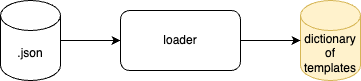
\includegraphics[scale=0.4]{./media/loader.png}
%    \caption{Loader}
%    \label{fig:load_templates}
%  \end{wrapfigure}
  Ingestion of the JSON, or internal data structures into an internal database that we call a \emph{registry}. Registries can be implemented as a \emph{dictionaries, maps} or \emph{databases}.
%
%\begin{verbatim}
 %   routings = json.loads(json_data)
%\end{verbatim}

\subsection{Instantiate system.}
%  \begin{wrapfigure}{l}{0.5\textwidth}
%    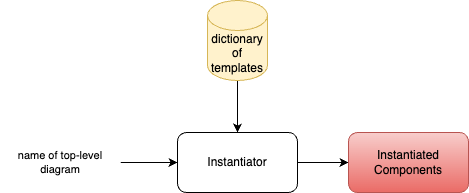
\includegraphics[scale=0.4]{./media/instantiate.png}
%    \caption{Instantiate}
%    \label{fig:instantiate_system}
%  \end{wrapfigure}

  Instantiation\cite{run} of an application beginning with a top-level diagram
and proceeds downwards to instantiate all children components needed in
the top-level diagram and, recursively, instantiating the childrens'
children. Components are instantiated based on their DPL templates.
Containers are instantiated by instantiating all child components and
all routings between components. Note that more than one child component
can refer to the same DPL template. Components must be uniquely
instantiated - typically their (x,y) position is enough to differentiate
components, but, \texttt{draw.io} assigns unique
id's to each template component, which we ended up using instead of
relying on (x,y) graphical information. Assigning unique id's is a
convenience, not a requirement, since the same information can be inferenced 
using multiple approaches.
%\begin{verbatim}
%main_container = get_component_instance(pregistry, main_container_name,  owner=None)
%\end{verbatim}
Software components are fully isolated from one another through the use
of FIFO queues.

\subsection{Inject first message.}
%  \begin{wrapfigure}{r}{0.5\textwidth}
%    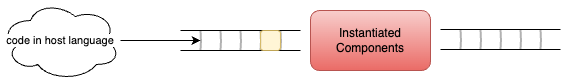
\includegraphics[scale=0.4]{./media/inject.png}
%    \caption{Inject first message(s)}
%    \label{fig:inject_first_message}
%  \end{wrapfigure}

The first message is constructed using the host language. The message is
injected\cite{main} into the input queue of the top-most component.
%
%\begin{verbatim}
%def start_function (root_project, root_0D, arg, main_container):
%   arg = new_datum_string (arg)
%   msg = make_message("", arg)
%    inject (main_container, msg)
%\end{verbatim}
  
\subsection{Run.}
%  \begin{wrapfigure}{m}{0.5\textwidth}
%    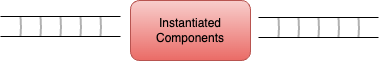
\includegraphics[scale=0.4]{./media/run.png}
%    \caption{Run}
%    \label{fig:run}
%  \end{wrapfigure}
The application is executed.

The application is interpreted by repeatedly delivering messages along
connections, recursively, until no messages remain in any input queues.

\emph{It is possible to invoke already-written library code written in some other host language using an activity indicator - see the code repo for more details.}

Containers must consume only one input message at a time while waiting
for all children to reach quiescence.
%
%\begin{verbatim}
%    if not load_errors:
%       injectfn (root_project, root_0D, arg, main_container)
%\end{verbatim}
  
\subsection{Display outputs.}
%  \begin{figure}[h]
%    \centering
%    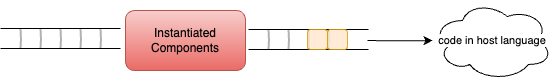
\includegraphics[scale=0.4]{./media/display.png}
%    \caption{Display Outputs}
%    \label{fig:display}
%  \end{figure}

The outputs in the output queue of the top-level component are displayed
using the host language.
%
%\begin{verbatim}
%   dump_outputs (main_container)
%\end{verbatim}
  

The Python version of the runtime system consists of roughly 9 files of
code consisting of about 2,500 lines of code (including blank lines and
comments) and is supported by a standard library consisting of another 5
files of code containing about 430 lines of code.

%At the basic level, runtime component instances are asynchronous, but,
%use named and anonymous functions and closures, instead of operating
%system processes. As such, programs written this way "feel" like
%\emph{programs} instead of as \emph{processes} in terms of efficiency.
Programs written this way "feel" like
\emph{programs} instead of as \emph{processes} in terms of efficiency because anonymous functions and closures are used instead of processes.

\section{Work In Progress}
We have built working examples of various other technologies, using the
DPL described in this paper, including,
\underline{VSH}\cite{vsh} a Visual SHell that works like /bin/sh pipelines employing more input and output ports,
\underline{arith0d}\cite{arith0d} OhmJS' arithmetic grammar that concurrently emits four (4) target languages (Javascript, Python, Common Lisp, WASM),
\underline{LLM0D}\cite{llm0d} a single component diagram that uses the Go programming language as a host language to connect to openai's LLM for experimenting with LLMs,
\underline{transpiler}\cite{transpiler} a workbench for creating new textual syntaxes, uses OhmJS more than once in a pipeline,
\underline{kinopio2md}\cite{k2m} experiment for converting Kinopio "mindmaps" into markdown based on connections between ideas expressed in Kinopio,
\underline{Scheme to Javascript}\cite{scm2js}, \underline{Scheme to Python}\cite{scm2py} - conversion of Nils Holm's Scheme code used in "Prolog Control Flow in 6 Slides" to produce a Prolog-like inferencing engine for Javascript, currently working on conversion to Python,
\underline{delay0d}\cite{delay0d},
\underline{dc0d}\cite{dc0d} game based on Chris Marten's "dungeon crawler" example\cite{ceptre_paper}; including gen0D generates components (in Odin) from the diagram (instead of interpreting the diagram, gen0D creates leaf components that are used in conjunction with the diagram),
\underline{0D odin}\cite{odin0d} a DPL engine written in the Odin programming language (Odin is statically typed, and, does not provide garbage collection, similar to languages like C),
\underline{Crystal 0D}\cite{crystal0d} a DPL engine written in the Crystal programming language, which is currently being used in a production system,
\underline{0D cookbook}\cite{0dcookbook} ongoing effort to document all standard DPL components as \href{http://draw.io}{draw.io} diagrams

\section{Fundamental Principles}
Software components are fully isolated from one another through the use
of FIFO queues. Using the LIFO callstack for inter-component
communication leads to hidden dependencies which leads to avoidance of
DPLs. This is a requirement for enabling LEGO®-like composition of software components.
FIFO-based callstacks only give the illusion of LEGO®-like composition of software libraries,
but, actually result in dynamic, tight coupling of components.

There must be exactly one input queue and one output queue per component. We
do not use, for semantic reasons, one queue per port. In general, single
queues allow programs to track relative time-ordering of messages - an
important feature when programming devices that perform sequencing
instead of computation. In addition, multiple queues can lead to
deadlock issues. These issues still exist in the large, but are
mitigated through the use of single input and output queues and tend not
to occur in hidden, unexpected ways.

Connections between components are triples that contain a routing direction.
There are four (4) kinds of routings as discussed in Section \ref{containerleaf}.
Routings are handled solely by parent Containers of components. Components, themselves, cannot route messages directly to other components, but, must leave output messages on their own output queues. Outputs are deferred, a parent Container of a component instance delivers the output messages, according to the routing connections, after the component has finished executing a step of its execution.


\section{Relevant Principles and Issues}
We do not discuss the following principles in detail in this paper, due
to reasons of space.

\emph{Structured Message Passing},
\emph{Rule of 7},
\emph{Parental Authority},
\emph{Asynchronicity and time-relative ordering},
\emph{SEND in addition to CALL},
\emph{Locality of Reference},
\emph{Scoping of names},
\emph{Children cannot change the behaviour of their parents},
\emph{CPUs are meant to be single-threaded},
\emph{Multiple happy paths of equal importance},
\emph{Subroutines are not functions},
\emph{Hidden dependencies},
\emph{Build-and-forget},
\emph{Breaking free of the function-based paradigm},
\emph{Building new paradigms using existing tools},
\emph{t2t - text-to-text transpilation pipelines},
\emph{Multiple syntaxes - notations - instead of general purpose programming languages},
\emph{Using existing GPLs as assemblers},
\emph{Writing code that writes code},
\emph{Inferencing semantic information from diagrams using various techniques},
\emph{Simple relations, like intersection, larger, smaller, above, below, left-of, right-of},
\emph{Low-level concepts like \emph{loop}, and \emph{recursion}, don't make sense in a distributed environment},
\emph{if-then-else is too low level and ad-hoc for expressing control-flow}.

\section{Future}
\begin{itemize}
\item Compilation, in addition to the interpretation, of DPLs.

\item Parsing XML using the \emph{Transpiler} component instead of calling XML parsing libraries.

\item Testing, unit testing, coverage testing.

\end{itemize}

\section{References}

\begin{thebibliography}{9}

\bibitem{diagrams_net}
Diagrams.net.
\url{https://app.diagrams.net}

\bibitem{ceptre_paper}
Martens, Chris. Ceptre: A Language for Modeling Generative Interactive Systems. \url{https://www.cs.cmu.edu/~cmartens/ceptre.pdf} (Accessed: January 19, 2024).

\bibitem{graphml}
\url{https://en.wikipedia.org/wiki/GraphML} (Accessed: April 22, 2024)

\bibitem{peg}
\url{https://en.wikipedia.org/wiki/Parsing_expression_grammar} (Accessed: April 22, 2024)

\bibitem{fortran}
\url{https://en.wikipedia.org/wiki/Fortran} (Accessed: April 22, 2024)

\bibitem{ohmjs}
\url{https://ohmjs.org} (Accessed: April 22, 2024)

\bibitem{odin}
\url{https://odin-lang.org} (Accessed: April 22, 2024)

\bibitem{d2j}
\emph{anonymous repository}

\bibitem{json}
\url{https://www.json.org/json-en.html} (Accessed: April 22, 2024)

\bibitem{d2jrepo}
\emph{anonymous repository}

\bibitem{run}
\emph{anonymous repository}

\bibitem{main}
\emph{anonymous repository}

\bibitem{vsh}
\emph{anonymous repository}

\bibitem{arith0d}
\emph{anonymous repository}

\bibitem{transpiler}
\emph{anonymous repository}

\bibitem{llm0d}
\emph{anonymous repository}

\bibitem{scm2js}
\emph{anonymous repository}

\bibitem{scm2py}
\emph{anonymous repository}

\bibitem{delay0d}
\emph{anonymous repository}

\bibitem{k2m}
\emph{anonymous repository}

\bibitem{odin0d}
\emph{anonymous repository}

\bibitem{dc0d}
\emph{anonymous repository}

\bibitem{crystal0d}
\emph{anonymous repository}

\bibitem{0dcookbook}
\emph{anonymous repository}

\end{thebibliography}

\end{document}
